\documentclass[10pt,a4paper,conference]{IEEEtran}

% Some very useful LaTeX packages include:
% (uncomment the ones you want to load)

% *** CITATION PACKAGES ***
%
\ifCLASSOPTIONcompsoc
  % IEEE Computer Society needs nocompress option
  % requires cite.sty v4.0 or later (November 2003)
  \usepackage[nocompress]{cite}
\else
  % normal IEEE
  \usepackage{cite}
\fi
% cite.sty was written by Donald Arseneau
% V1.6 and later of IEEEtran pre-defines the format of the cite.sty package
% \cite{} output to follow that of IEEE. Loading the cite package will
% result in citation numbers being automatically sorted and properly
% "compressed/ranged". e.g., [1], [9], [2], [7], [5], [6] without using
% cite.sty will become [1], [2], [5]--[7], [9] using cite.sty. cite.sty's
% \cite will automatically add leading space, if needed. Use cite.sty's
% noadjust option (cite.sty V3.8 and later) if you want to turn this off.
% cite.sty is already installed on most LaTeX systems. Be sure and use
% version 4.0 (2003-05-27) and later if using hyperref.sty. cite.sty does
% not currently provide for hyperlinked citations.
% The latest version can be obtained at:
% http://www.ctan.org/tex-archive/macros/latex/contrib/cite/
% The documentation is contained in the cite.sty file itself.
%
% Note that some packages require special options to format as the Computer
% Society requires. In particular, Computer Society  papers do not use
% compressed citation ranges as is done in typical IEEE papers
% (e.g., [1]-[4]). Instead, they list every citation separately in order
% (e.g., [1], [2], [3], [4]). To get the latter we need to load the cite
% package with the nocompress option which is supported by cite.sty v4.0
% and later. Note also the use of a CLASSOPTION conditional provided by
% IEEEtran.cls V1.7 and later.


% *** GRAPHICS RELATED PACKAGES ***
%
  \usepackage[pdftex]{graphicx}
  \graphicspath{{../Figures/}}
  \DeclareGraphicsExtensions{.pdf,.png}
  \usepackage{color}

% *** MATH PACKAGES ***
%
\usepackage[cmex10]{amsmath}
% A popular package from the American Mathematical Society that provides
% many useful and powerful commands for dealing with mathematics. If using
% it, be sure to load this package with the cmex10 option to ensure that
% only type 1 fonts will utilized at all point sizes. Without this option,
% it is possible that some math symbols, particularly those within
% footnotes, will be rendered in bitmap form which will result in a
% document that can not be IEEE Xplore compliant!
%
% Also, note that the amsmath package sets \interdisplaylinepenalty to 10000
% thus preventing page breaks from occurring within multiline equations. Use:
%\interdisplaylinepenalty=2500
% after loading amsmath to restore such page breaks as IEEEtran.cls normally
% does. amsmath.sty is already installed on most LaTeX systems. The latest
% version and documentation can be obtained at:
% http://www.ctan.org/tex-archive/macros/latex/required/amslatex/math/

%\usepackage{amssymb}%............................ AMS Symbol fonts



% *** SPECIALIZED LIST PACKAGES ***
%
%\usepackage{algorithmic}
% algorithmic.sty was written by Peter Williams and Rogerio Brito.
% This package provides an algorithmic environment for describing algorithms.
% You can use the algorithmic environment in-text or within a figure
% environment to provide for a floating algorithm. Do NOT use the algorithm
% floating environment provided by algorithm.sty (by the same authors) or
% algorithm2e.sty (by Christophe Fiorio) as IEEE does not use dedicated
% algorithm float types and packages that provide these will not provide
% correct IEEE style captions. The latest version and documentation of
% algorithmic.sty can be obtained at:
% http://www.ctan.org/tex-archive/macros/latex/contrib/algorithms/
% There is also a support site at:
% http://algorithms.berlios.de/index.html
% Also of interest may be the (relatively newer and more customizable)
% algorithmicx.sty package by Szasz Janos:
% http://www.ctan.org/tex-archive/macros/latex/contrib/algorithmicx/

% *** ALIGNMENT PACKAGES ***
%
\usepackage{array}
% Frank Mittelbach's and David Carlisle's array.sty patches and improves
% the standard LaTeX2e array and tabular environments to provide better
% appearance and additional user controls. As the default LaTeX2e table
% generation code is lacking to the point of almost being broken with
% respect to the quality of the end results, all users are strongly
% advised to use an enhanced (at the very least that provided by array.sty)
% set of table tools. array.sty is already installed on most systems. The
% latest version and documentation can be obtained at:
% http://www.ctan.org/tex-archive/macros/latex/required/tools/


\usepackage{mdwmath}
\usepackage{mdwtab}
% Also highly recommended is Mark Wooding's extremely powerful MDW tools,
% especially mdwmath.sty and mdwtab.sty which are used to format equations
% and tables, respectively. The MDWtools set is already installed on most
% LaTeX systems. The lastest version and documentation is available at:
% http://www.ctan.org/tex-archive/macros/latex/contrib/mdwtools/

% IEEEtran contains the IEEEeqnarray family of commands that can be used to
% generate multiline equations as well as matrices, tables, etc., of high
% quality.

% *** SUBFIGURE PACKAGES ***
\ifCLASSOPTIONcompsoc
  \usepackage[caption=false,font=normalsize,labelfont=sf,textfont=sf]{subfig}
\else
  \usepackage[caption=false,font=footnotesize]{subfig}
\fi

%Setting captions to centered (Not IEEE journal standard)
%\makeatletter
%\long\def\@makecaption#1#2{\ifx\@captype\@IEEEtablestring%
%\footnotesize\begin{center}{\normalfont\footnotesize #1}\\
%{\normalfont\footnotesize\scshape #2}\end{center}%
%\@IEEEtablecaptionsepspace
%\else
%\@IEEEfigurecaptionsepspace
%\setbox\@tempboxa\hbox{\normalfont\footnotesize {#1.}~~ #2}%
%\ifdim \wd\@tempboxa >\hsize%
%\setbox\@tempboxa\hbox{\normalfont\footnotesize {#1.}~~ }%
%\parbox[t]{\hsize}{\normalfont\footnotesize \noindent\unhbox\@tempboxa#2}%
%\else
%\hbox to\hsize{\normalfont\footnotesize\hfil\box\@tempboxa\hfil}\fi\fi}
%\makeatother


% *** FLOAT PACKAGES ***
%
\usepackage{fixltx2e}
% fixltx2e, the successor to the earlier fix2col.sty, was written by
% Frank Mittelbach and David Carlisle. This package corrects a few problems
% in the LaTeX2e kernel, the most notable of which is that in current
% LaTeX2e releases, the ordering of single and double column floats is not
% guaranteed to be preserved. Thus, an unpatched LaTeX2e can allow a
% single column figure to be placed prior to an earlier double column
% figure. The latest version and documentation can be found at:
% http://www.ctan.org/tex-archive/macros/latex/base/

% *** PDF, URL AND HYPERLINK PACKAGES ***
%
\usepackage{url}

\usepackage{sistyle}
    \SIstyle{S-Africa}
    \SIunitspace{{\cdot}}
    \SIunitdot{{\cdot}}

% generate nice bookmarks and hyperrefs when exporting to pdf and dvi (screen version):
\usepackage[a4paper,plainpages=false,colorlinks,linktocpage,bookmarks=true,bookmarksopen=false]{hyperref}
% use this for printing only (no color, print version):
%\usepackage[a4paper,plainpages=false,colorlinks=false,linktocpage,bookmarks=true,bookmarksopen=false]{hyperref}

% correct bad hyphenation here
\hyphenation{op-tical net-works semi-conduc-tor}

%Add elegant support for Big-O notation
\providecommand{\OO}[1]{\operatorname{O}\left(#1\right)}

\begin{document}

%
% paper title
\title{Pithos: A State Persistency Architecture for Peer-to-Peer Massively Multiuser Virtual Environments}

%\author{\IEEEauthorblockN{John S. Gilmore and Herman A. Engelbrecht\\}
%\IEEEauthorblockA{MIH Media Lab\\
%Electronic Engineering Department\\
%Stellenbosch University\\
%Stellenbosch, South Africa\\
%mail: jgilmore@ml.sun.ac.za and hebrecht@sun.ac.za}}

\maketitle

\begin{abstract}
%\boldmath
The field of state persistency for peer-to-peer massively multiuser virtual environments (PMMVEs) is explored and categorised into super peer
storage, overlay storage, hybrid storage and distance-based storage. The storage types are briefly evaluated against the identified storage system
requirements of scalability, fairness, reliability, responsiveness and security. All storage types are found to be lacking in some respects and
therefore a novel storage system called Pithos is introduced. The design of Pithos, which is based on a multi-tiered hybrid architecture making use
of grouping is presented. Preliminary results show that Pithos addresses all of the identified requirements.

\end{abstract}


\section{Introduction}
\label{introduction}

%P2P MMVE Background
Peer-to-Peer (P2P) Massively Multiuser Virtual Environments (MMVEs) have received significant attention from the research community, since the first
publication on the subject by Knutssonn et al. in 2004 \cite{knutsson_p2p_first}. P2P MMVEs promise to solve many issues prevalent in today's
Client/Server (C/S) based MMVEs. Some key issues have to be solved before P2P MMVEs can be implemented commercially.

%Key challenges and focus
Recently, six key challenges of P2P systems have been identified: \emph{interest management}, \emph{game event dissemination}, \emph{non-player
character (NPC) host allocation}, \emph{game state persistency}, \emph{cheating mitigation} and \emph{incentive mechanisms}
\cite{Fan_deisgn_issues_p2p}. Most of the challenges mentioned have received significant attention from the research community, with the exception of
state persistency.

State persistency defines how object states should be stored. Objects states can be anything from a user's position to the state of the virtual
market in an MMVE. For a P2P MMVE, game data must be distributed amongst various peers in the network. This creates challenges not usually present in
classic C/S MMVEs. The focus of this paper is exclusively on state persistency in P2P MMVEs.

%Current techniques not perfect
The paper first attempts to categorise state persistency mechanisms found in the literature. The paper then shows that thus far none of the
approaches to state persistency meet the storage requirements of modern MMVEs. All storage models are evaluated according to the identified
requirements of scalability, fairness, reliability, responsiveness and security.

%Propose multi-tiered model
Because current state persistency models do not address all the requirements of modern MMVEs, a novel hybrid multi-tiered state persistency model is
proposed, called Pithos

%Implementation
The proposed multi-tiered model is currently being implemented in Oversim, a P2P simulation environment based in Omnet++. The model allows for the
measurement of the requirements identified. Furthermore, it allows for the comparison of the current model with other state persistency models.
Initial results seem promising, with the implemented model functioning as expected. The system shows to be very responsive when storing data within a
group and as responsive as storing data in an overlay when storing data between groups.

%TODO: This should be reviewed
%Summary
Section \ref{current_models} groups storage models found in the literature and describes the advantages and disadvantages of each group.
%
In Section \ref{design} a novel state persistency architecture design is described.
%
Section \ref{evaluation} presents an evaluation of the proposed state persistency model and presents some preliminary results.
%
Section \ref{conclusion} concludes with a summary of the paper and a discussion on possible future work.

\section{Distributed state persistency models}
\label{current_models}

%Overview of four approaches
After reviewing various storage architectures, we were able to categorise the reviewed architectures into four broad types by which state persistency
is achieved in P2P MMVEs. These are: \emph{super peer storage}, \emph{overlay storage}, \emph{distance-based storage} and \emph{hybrid storage}. In
order to evaluate the different storage types, we identified the following requirements:

\begin{itemize}
%Scalability
\item \emph{Scalability}: For an MMVE state persistency architecture to be scalable, it should be able to support thousands of users. In the
    paper, scalability it not handled as some separate entity, but rather all other requirements are evaluated in terms of a system of thousands
    of users.

%Reliability
\item \emph{Reliability}: Reliability is defined to mean that a file in the storage system may neither be lost, nor be unavailable when a user
    requests it.

%Fairness
\item \emph{Fairness}: For a system to be fair, the responsibility of storage should be equally shared amongst all users according to their
    available resources. This ensures that costs due to bandwidth and storage are shared amongst all.

%Responsiveness
\item \emph{Responsiveness}: Responsiveness is a requirement that has not really been part of file storage systems in the past. For games, it is
    believed that responsive object storage is a key requirement to promote responsive game play and robust recovery mechanisms.

%Security
\item \emph{Security} Data security is a major issue for distributed storage, because data are stored on users' machines who should not
    necessarily be able to access and alter the data stored.
\end{itemize}

\begin{table}[htbp]
\centering
\begin{tabular}{|r|c|c|c|c|}
\hline
Storage type & Reliability & Responsiveness & Security & Fairness\\
\hline
Super Peer & Medium & High & Low & Low\\
Overlay & High & Low & Medium & High\\
Hybrid & High & High & Medium & Low\\
Distance & Medium & High & Low & Medium\\
\hline
\end{tabular}
\caption{Differences between storage mechanisms} \label{tab_storage}
\end{table}
%
Table \ref{tab_storage} presents a characterisation of current storage systems according to the characteristics defined. Table \ref{tab_storage} also
provides some references that act as examples of the different storage types mentioned.

\subsection{Super peer storage}

%Super peer storage - description
Super peer storage relies on the super peer storing all information that is in its domain \cite{knutsson_p2p_first}. A domain is usually created by
segmenting the world into regions and super peers act as regional servers to all peers in their region. Each super peer handles state persistency for
its region, hosting NPCs, objects and persistent player data. This storage method is much like a Client/Server setup, with the super peer acting as
the server for the virtual geographic region assigned to it.

The advantage of super peer storage is that it's responsive. The disadvantages of super peer storage stem from the per-region centralised approach,
where super peers have access to all region data and they are the only entities in the network that store data. This leads to the main issues with
super peer storage being lack fairness and security. It is also difficult to achieve high levels of reliability.


\subsection{Overlay storage}

%Description
Overlay storage is classified as using any type of structured P2P overlay to store data in a distributed fashion \cite{Douglas05enablingmassively},
\cite{using_freenet_storage}, \cite{Fan_phd}, \cite{past_storage_focus}. This is a very broad definition, which basically encompasses any P2P
distributed storage currently in use. Some examples and a comparison of different distributed storage techniques can be found in
\cite{Hasan_distributed_storage_survey}.

%Advantages/Disadvantages
Overlay storage is characterised by all nodes sharing all objects as well as multiple replicas of those objects and a storage time of $O(\log(N))$,
where $N$ is the total number of nodes in the network. From this follows the main advantages of overlay storage being reliability, fairness and
reasonable security, with the main disadvantage being lack of responsiveness.

\subsection{Hybrid storage}

%Description
The world is divided into regions, with each region controlled by a super peer \cite{zoned_federation}, \cite{hybrid_storage1}. The complete region
state is cached at every super peer, the same as with super peer storage. There also exists a backup overlay storage architecture, to which data may
be backed up for long term, redundant and secure storage.

%Advantages/Disadvantages
Hybrid storage combines some of the features present in overlay and super peer storage to have the advantages of high reliability from overlay
storage and high responsiveness from super peer storage. Hybrid storage, does however, still suffer from the same security issues and lack of
fairness present in super peer storage.

\subsection{Distance-based storage}
\label{classic_distance_based}

%Description
Distance based approaches, such as the Voronoi storage approaches \cite{Buyukkaya_voronoi_state_management}, \cite{Hu_voronoi_IM} and some more
general approaches \cite{colyseus_distance_based}, \cite{solipsis}, store object data on the peer closest to the object in the virtual world. In some
systems, only player states are considered for storage \cite{individual_storage1}, \cite{cheat_proof_playout}. This storage type is termed individual
storage and is considered as a subset of distance-based storage, which also allows for non-player objects to be stored.

%Advantages/Disadvantages
Distance-based storage exploits the assumption that objects close to each other in the virtual world are more likely to interact with one another and
that the number of objects stored per nodes depends on the distribution of nodes in the virtual world. This leads to responsiveness being the main
advantage of distance-based storage, but the disadvantages being lack of reliability and security and that it can suffer from some fairness issues.

\subsection{Summary and comparison}

From this discussion, it is evident that none of the mentioned storage types in their current forms are appropriate for data storage in MMVEs. Super
peer storage is not fair or secure, overlay storage is not responsive, hybrid overlay/super peer storage is not fair and distance-based storage is
not secure and not yet reliable.

It should also be noted that most of these storage types are not mature. In the referenced papers, they were mentioned as a means by which
persistency might be achieved. But none of the papers, save for PAST \cite{storage_and_chaching_PAST}, presented concrete designs and results.

This shows that not only is a storage type required that improves upon previous storage types, but a concrete design and implementation is also
required that uncovers unforeseen issues that might arise when implementing P2P MMVEs. The following section attempt to provide such a design.

\section{Architecture design}
\label{design}

In this section ``Pithos'', the proposed P2P MMVE state persistency architecture design is described. The inspiration for this architecture comes
from two observations:
%
\begin{enumerate}
  \item One can combine multiple storage models and arrive at a model which possesses fewer disadvantages than any of the models used.
  \item Responsiveness is greatly increased in a fully distributed model, where there is no intermediate server that relays all information. It
      was, however, also observed that fully distributed architectures are not scalable because of the number of messages scaling by an $O(N^2)$,
      where $N$ is the number of nodes in the network.
\end{enumerate}

\begin{figure}[htbp]
 \centering
 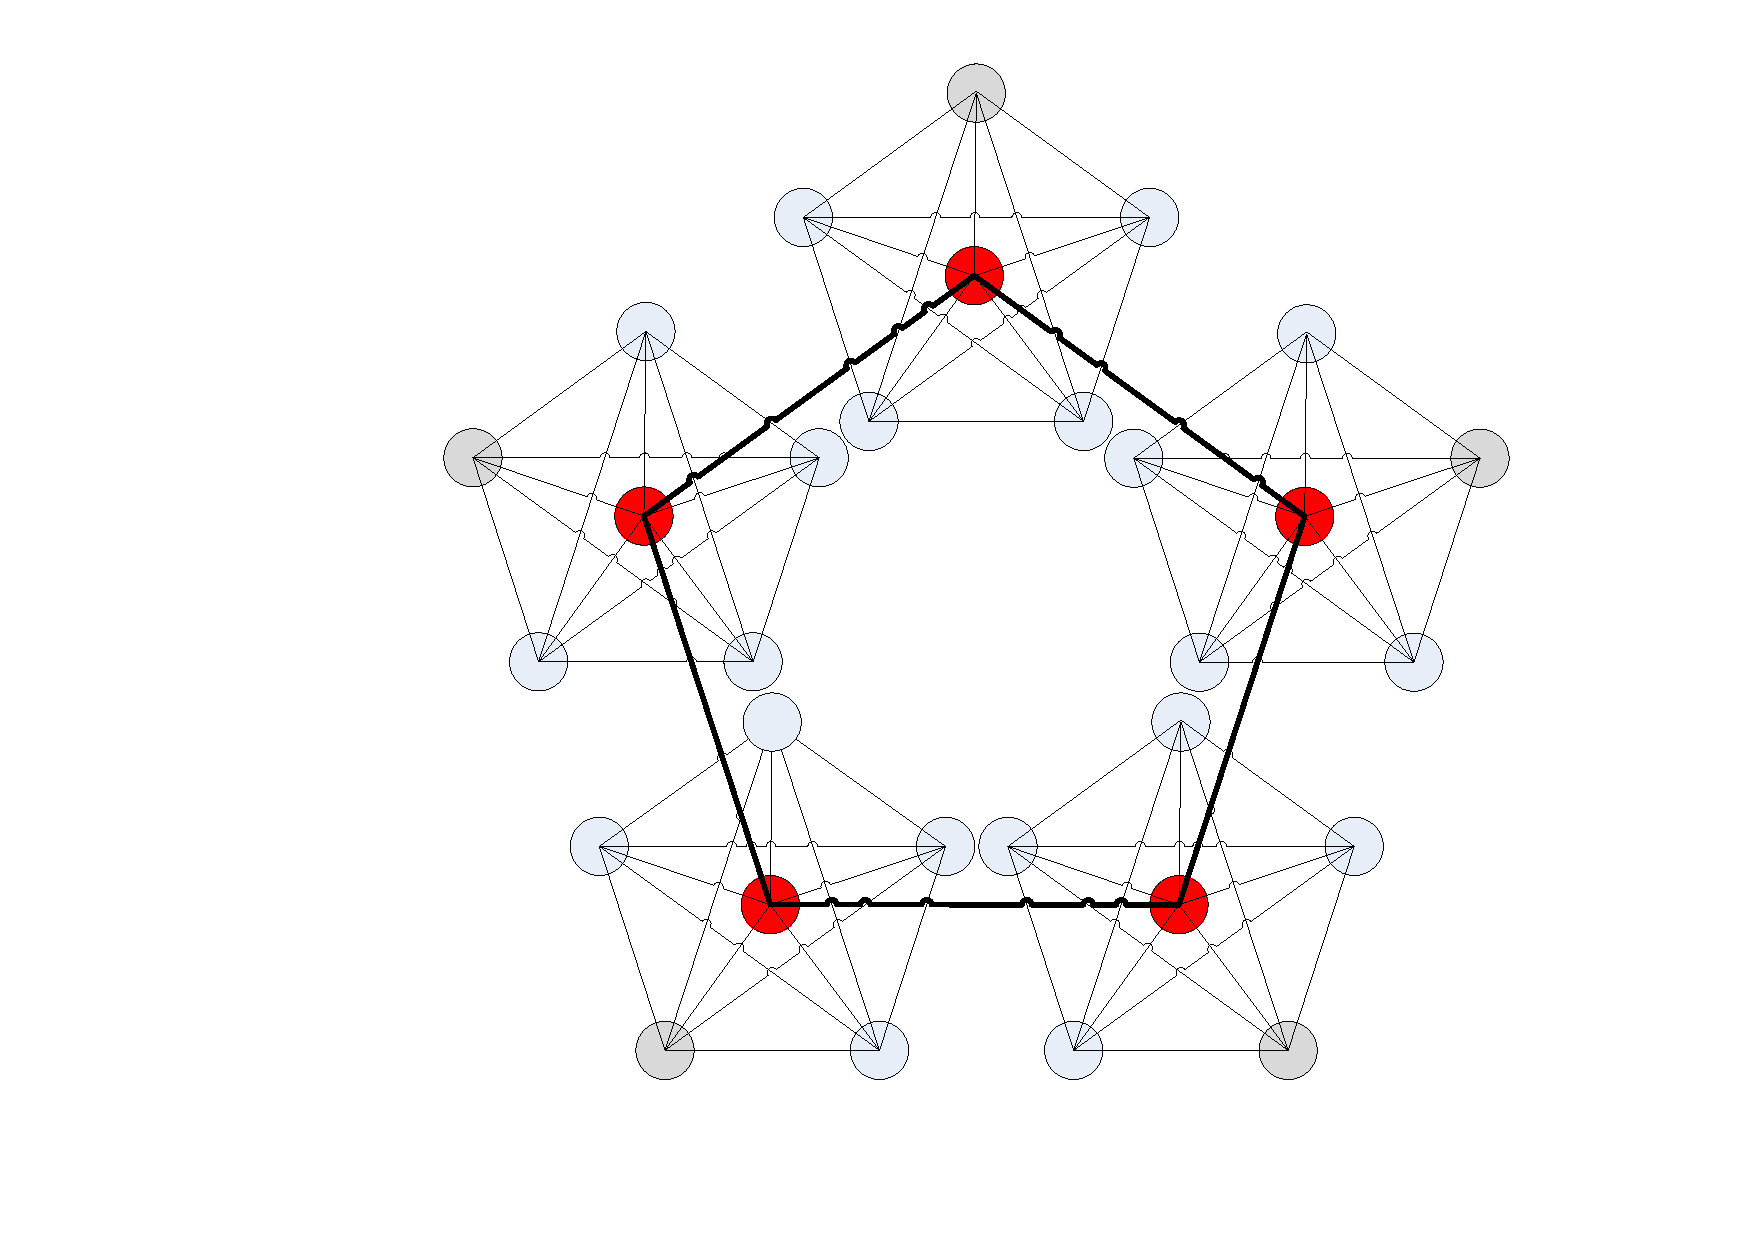
\includegraphics[clip=true, viewport=7.5cm 2.5cm 26cm 20cm, width=0.7\columnwidth]{CDHT_layout}
 \caption{Layout of the Pithos storage architecture}
 \label{fig_pithos}
\end{figure}
%
Figure \ref{fig_pithos} shows the Pithos architecture. The figure shows groups of fully connected peers (blue and red), where all groups are
connected to each other in an P2P overlay through super peers (red).

Pithos groups peers in some way to form a two tiered storage model. The first tier is a storage model at group level and the second is a model over
all groups. On the first tier, which is the intra-group level, a fully distributed storage system is used to allow for highly responsive read and
write operations within the group. On the second tier, which is the inter-group level, a P2P overlay is used to store data between groups.

\subsection{Grouping}

%Speak more concretely of grouping algorithms
At the core of the architecture is how peers are grouped. Two approaches are being evaluated to group peers, one is by using distributed clustering
techniques, for example affinity propagation \cite{affinity_propagation}, the other is by using dynamic regioning techniques, for example
self-organising spatial publish subscribe (SOSPS) \cite{self_organising_sps_post}.

Distributed clustering techniques will make use of the flocking behaviour of players to dynamically group players into flocks or clusters
\cite{flocking}. The main idea of flocking is that players move around in groups, rather than randomly on their own. Because of the flocking
behaviour of players, dynamic groups or regions that move with groups of players may be a better fit than static or even dynamic regions that operate
on areas of the virtual world and not on how groups of players actually cluster. Because a fully distributed architecture is not scalable, player
density within groups should remain constant. This means that groups should merge or split as the player density within them change.

Affinity propagation clusters nodes using a similarity matrix to find similar nodes. The similarity matrix may contain any type of quantity and can
contain player positions. Affinity propagation will then group nodes depending on their location in a virtual world. This algorithm is ideally suited
to P2P applications, since it is a distributed clustering algorithm based on message passing.

As an alternative to clustering, dynamic regioning might also be used to group players. SOSPS is a new and promising development in dynamic
regioning. SOSPS creates dynamic regions based on a Voronoi overlay network \cite{voronoi_diagrams_survey}. Near constant player density is achieved
by increasing and decreasing the area sizes. This system is based on VON, a distributed Voronoi overlay network designed for MMVEs \cite{VON_VAST}.

\subsection{Store and retrieve with replication}
\label{store_retrieve}

The process of storing a file in Pithos is as follows:
\begin{enumerate}
\item A peer receives a store request from the higher game layer, along with the object that should be stored and an SHA-1 hash of that object.
\item The storing peer then replicates the object $k$ times.
\item For each object, the storing peer selects a single peer from its list of group peers by sampling from a uniformly random distribution.
\item Each object is then sent to the selected peer for storage.
\item The storing peer also sends an update message to all group peers to inform them of the new object available in the group and on which peers
    the object is stored.
\item The storing peer then sends an additional replica of the object to the super peer, along with a value ($l$) specifying how many overlay
    replicas are required.
\item The group super peer uses the received uniformly distributed SHA-1 hash as the destination ID to route the overlay object to.
\item The destination super peer received the overlay object and resends it to $l$ of its overlay neighbours.
\item At each destination super peer, the super peer selects a single node in its group from a uniform random distribution where the overlay
    object is then sent to and stored.
\end{enumerate}

Currently, Pithos sends the object with the store request to the group super peer, where the group super peer then forwards that object to another
super peer and that super peer then sends the object to a group peer for storage. A future improvement might be to only send signalling messages to
the nodes in the forwarding path that indicate that a source node has an object to store. When the signalling messages then arrive at the different
destination nodes, they can contact the source node directly and obtain the object from that node. This will reduce the amount of bandwidth consumed
by the storage operation.

The process of retrieving a file from Pithos is as follows:
\begin{enumerate}
\item A peer receives a retrieve request from the higher game layer that contains the object ID generated from the SHA-1 hash.
\item The peer then searches for the object in its list of group objects.
\item If the object is available in the group, the object is requested from the peer containing it and sent up to the game layer.
\item If the object is not available in the group, an object request is sent to the group super peer.
\item The group super peer requests the object by ID, forwards the received object to the requesting peer where the requesting peer then sends
    the object to the game layer.
\end{enumerate}

Pithos implements data replication to enable it to handle node churn. If a node leaves the network and stops to transmit pong messages, the migration
mechanism will detect this and replicate the file on another node. Replication exists intra- as well as inter-group and is useful in ensuring that if
a nodes leaves the network, the data is not lost. Because of how overly routing functions, if the root peer leaves, all object requests are routed to
the peer with the next closest ID. Because Pithos stores overlay replicas at overlay neighbours, the new destination peers will possess the stored
files.

\subsection{Secure storage and node ID assignments}
\label{secure_ids}

In order to design a secure distributed storage system, one requirement for the P2P overlay is that nodes should not be able to select their own IDs
or it will not be possible to secure the system against attack. Node IDs should rather be assigned securely by some certification authority
\cite{secure_overlay_routing}.

To this end Pithos implements its own certification authority to assign node IDs securely and promote security in the P2P overlay. A certification
server exists that handle ID requests from nodes. The server assigns IDs to nodes and provides the node with a signed certificate that it may use to
store data.

Whenever an object is stored or updated in the storage network, nodes have to sign the object to enable the tracking of object changes throughout the
life of the object. This system is very different from classic distributed file storage designs that advocate anonymity in storage. The fact that all
changes can be tracked to a specific node will simplify the task of eliminating player cheating.

\subsection{Distance-based storage} \label{distance_based}

For Pithos to perform well as an MMVE storage architecture, intra-group data requests should be preferred to inter-group data requests. This
requirement, combined with the fact that the grouping algorithm geographically groups players, lends Pithos to a storage system based on
distance-based storage. The assumption made is much the same as the one made for interest management, that players have a limit area of interest and
require interaction with a limited number of objects within range.

The design is then to implement distance-based storage, but on a group level rather than an individual level. This means that objects are stored on
the nearest group of players, rather than the nearest player. It is supposed that such an approach will also alleviate many of the challenges present
with distance-based storage.

With group-based distance-based storage, it is assumed that because peers now store objects closest to the group, the objects that they are
interested in will most likely be stored within their own group. What follows is that most data requests should be intra-group requests. The overlay
storage component ensures that nodes that require data not stored within their group are still able to access the data.

\section{Architecture evaluation}
\label{evaluation}

Pithos is currently still a work in progress, and although the design presented in the previous section is meant to address all identified
requirements, only preliminary results for responsiveness and fairness is presented in this section.

\subsection{Test setup}
\label{test_setup}

Pithos is being implemented in Oversim, running on Omnet++. Oversim was chosen because of the variety of already implemented protocols as well as the
layered architecture, which simplifies testing with different overlays and comparison with different storage types.

In the results shown, Pastry was used as the P2P overlay and Pithos was driven by a \emph{game} module. After a node has joined a group, the game
module starts to generate store and retrieve requests at a mean rate of 100 ms and a mean size of 1 KB, both sampled from exponential distributions.
Pithos was configured to store two group replicas and one overlay replica for every root object stored to give a ratio of group storage to overlay
storage of 3:1. The choice of these values is discussed in Section \ref{future_work}.

For the results shown in Section \ref{results}, 14999 peers, 4999 super peers and a single directory server are created at the start of the
simulation. The directory server publishes super peer information, which allows a peer to join the group nearest to it. Because of the way Pithos is
structured, each super peer node is also a peer node, which then gives a total of 15000 Oversim nodes.

\subsection{Responsiveness}

In the storage system, we expect two levels of responsiveness. We expect a certain level of responsiveness for intra-group communications and a
certain level of responsiveness for inter-group communications. We can calculate an average response time which is determined by the percentage of
intra-group requests, compared to inter-group requests as follows:
%
\begin{equation}\label{expected_response_time}
    E[T_{\textrm{resp}}] = P(g)\left(E\left[T_{\textrm{group}}\right]\right) + \left(1 - P(g)\right)\left(E\left[T_{\textrm{overlay}}\right]\right)
\end{equation}
%
, where $E[T_{\textrm{resp}}]$, the!carium0
 expected value of the overall system response time is given by $P(g)$, the probability that a message is
routed within a group, $E\left[T_{\textrm{group}}\right]$, the expected value of the root and replica message distribution as shown in Figure
\ref{fig_pithos_response} and $E\left[T_{\textrm{overlay}}\right]$, the expected value of the overly message distribution also shown in Figure
\ref{fig_pithos_response}.

\begin{figure}[htbp]
 \centering
 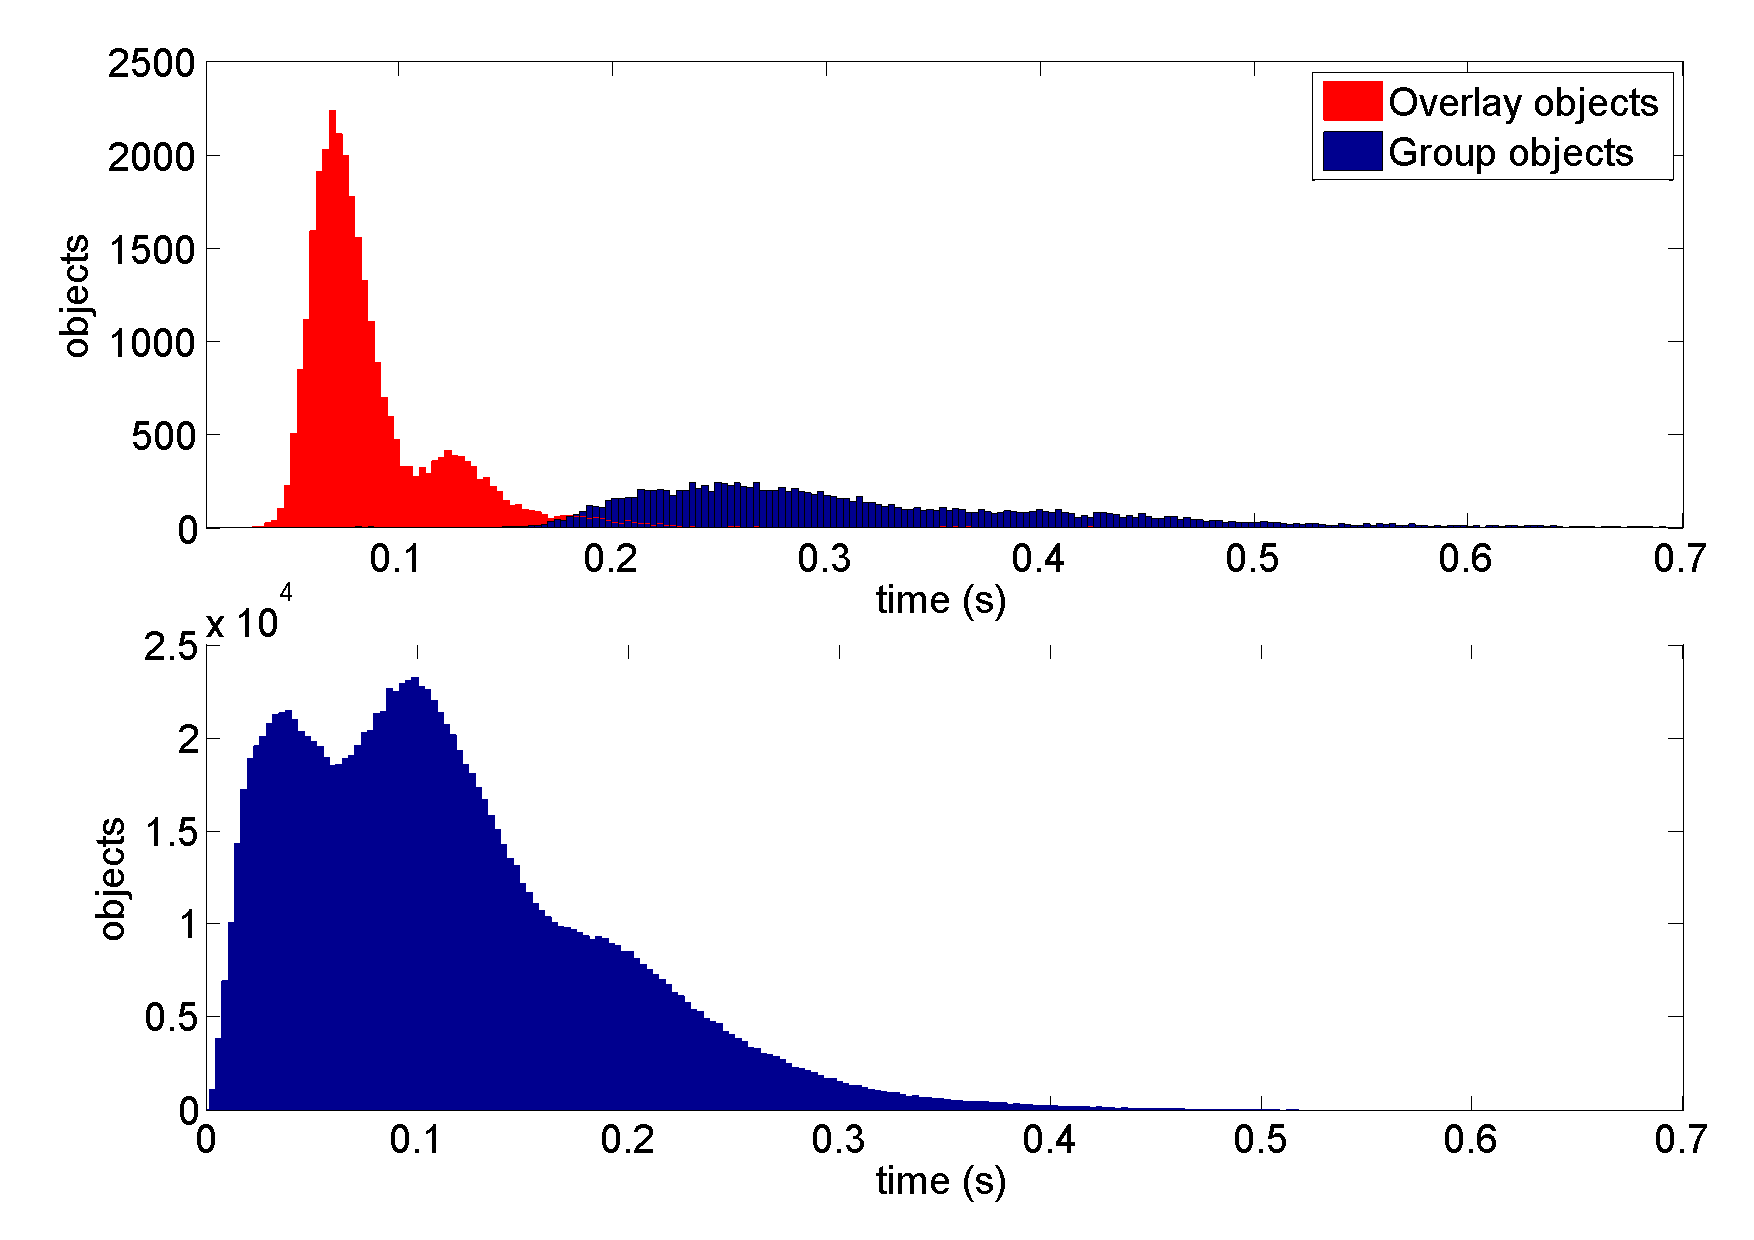
\includegraphics[clip=true, viewport=1cm 0.5cm 29cm 20.5cm, width=\columnwidth]{StoreTimes}
 \caption{Time distribution of overlay and root/replica objects}
 \label{fig_pithos_response}
\end{figure}
%
Figure \ref{fig_pithos_response} (top) shows the distribution of mean storage request times over all nodes in the Pithos network for the different
storage types. One can see that the intra-group root and replica objects are stored much faster ($E\left[T_{\textrm{group}}\right] = 0.0878 s$) than
the overlay objects in the network ($E\left[T_{\textrm{overlay}}\right] = 0.3284 s$).

From Figure \ref{fig_pithos_response} (top) it is evident that if only overlay storage is used, the storage and retrieval times will be much higher.
Figure \ref{fig_pithos_response} (bottom) presents the responsiveness of a pure Pastry network of 14999 nodes, using the \verb.KBRTestApp.
application and Pastry overlay in Oversim. The Pastry network has a mean routing time of 0.12 s. To exactly compare Pithos with overlay storage, the
percentage of intra-group requests ($P(g)$) should first be known. At this time there is no way to know what this percentage is, but the
responsiveness can be calculated as a function of $P(g)$.

The responsiveness of Pithos will depend on the responsiveness of Pastry, where the expected number of Pastry hops are given by
\cite{storage_and_chaching_PAST}:
%
\begin{equation}\label{pastry_hops}
    E[H_{\textrm{pastry}}] = \log_{2^b}\left(N\right)
\end{equation}
%
, where $b$ is a network parameter that is usually chosen as $b = 4$. From this, it is possible to calculate a theoretical performance for Pithos and
compare that with a theoretical performance of overlay storage.

When using a weighted hop average, as with Equation \eqref{expected_response_time}, the expected number of Pithos hops is given by:
%
\begin{equation}\label{expected_response_time}
    E[H] = P(g)\left(E\left[H_{\textrm{group}}\right]\right) + \left(1 - P(g)\right)\left(E\left[H_{\textrm{overlay}}\right]\right)
\end{equation}
%
, where $E\left[H_{\textrm{group}}\right]$ is the expected number of group hops and $E\left[H_{\textrm{overlay}}\right]$ is the expected number of
overly hops. In Pithos, $E\left[H_{\textrm{group}}\right] = 1$, because in a fully connected group any node is always one hop away from any other
node.

To find the value of $E\left[H_{\textrm{overlay}}\right]$, one has to look at how many hops an overlay message requires in Pithos. One hop is
required to send a store request from a group peer to its super peer. The super peer then forwards the message to another super peer in
$\log_{16}(M)$ hops, from Equation \eqref{pastry_hops}, where $M$ is the number of super peers in the network. From the destination super peer,
another hop is required to send the message to the destination group peer. This gives:
%
\begin{equation}\label{group_hops}
    E\left[H_{\textrm{group}}\right] = 1 + \log_{16}(M) + 1.
\end{equation}
%
Equation \eqref{expected_response_time} then becomes:
%
\begin{equation}\label{expected_response_time_exp}
    E[H] = P(g) + \left(1 - P(g)\right)\left(2 + \log_{16}\left(M\right)\right).
\end{equation}

\begin{figure}[htbp]
 \centering
 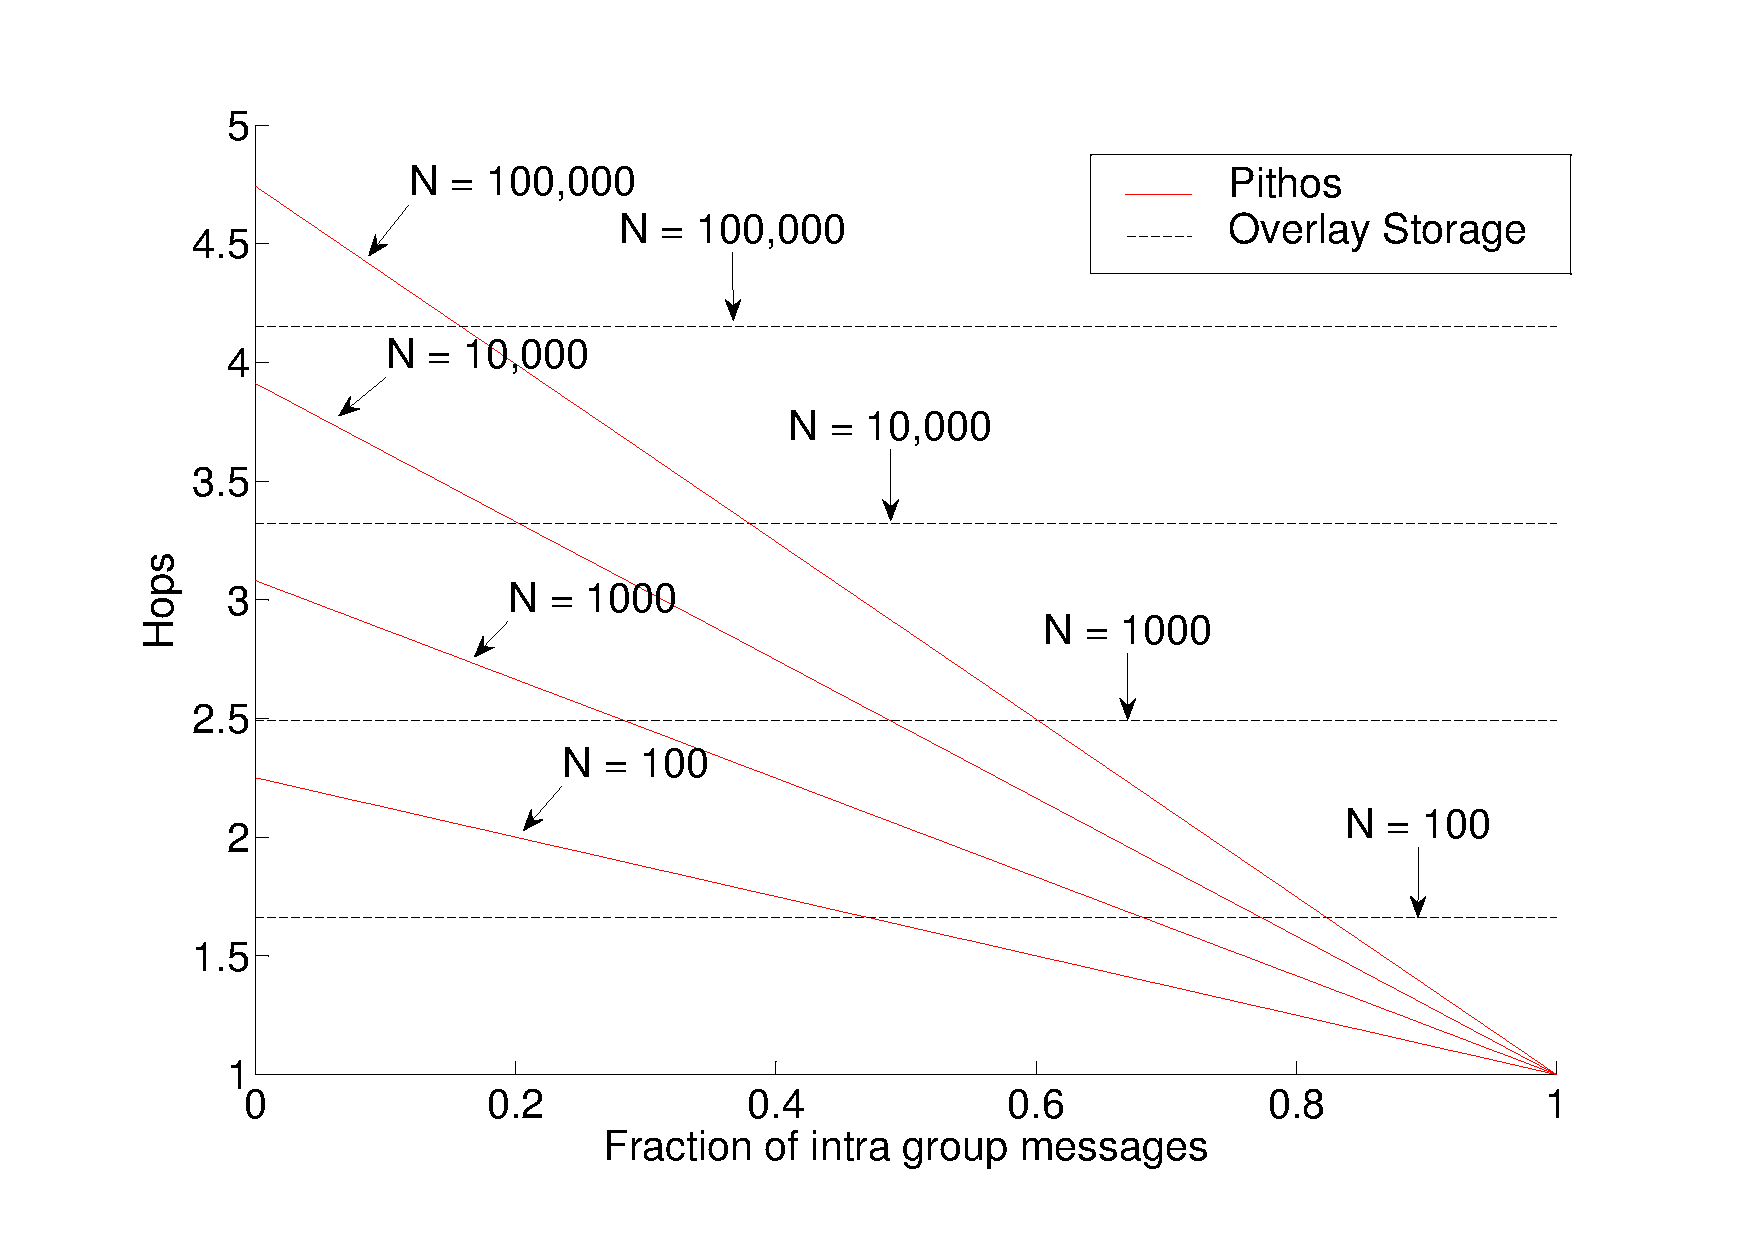
\includegraphics[clip=true, viewport=0cm 5cm 27cm 14.5cm, width=\columnwidth]{Hops_vsGroupFrac_4n}
 \caption{Time distribution of overlay and root/replica objects}
 \label{fig_hop_compare}
\end{figure}
%
Figure \ref{fig_hop_compare} compares the expected number of Pithos hops with the expected number of overlay hops as a function of intra-group
probability ($P(g)$) for various numbers of nodes ($N$). The overlay hops were calculated from Equation \eqref{pastry_hops}, while the Pithos hops
were calculated from Equation \eqref{expected_response_time_exp}. For the Pithos graphs, an average number of 50 peers per group was used to
determine the number of super peers.

Figure \ref{fig_hop_compare} shows that for a low value of $P(g)$, overlay storage performs better than Pithos because of the additional two hops
present in Pithos. Because of the distance-based design of Pithos that attempts to maximise the value of $P(g)$, high values for $P(g)$ are expected,
which means that the system is expected to perform better than overlay storage.

\subsection{Fairness}

\begin{figure}[htbp]
 \centering
 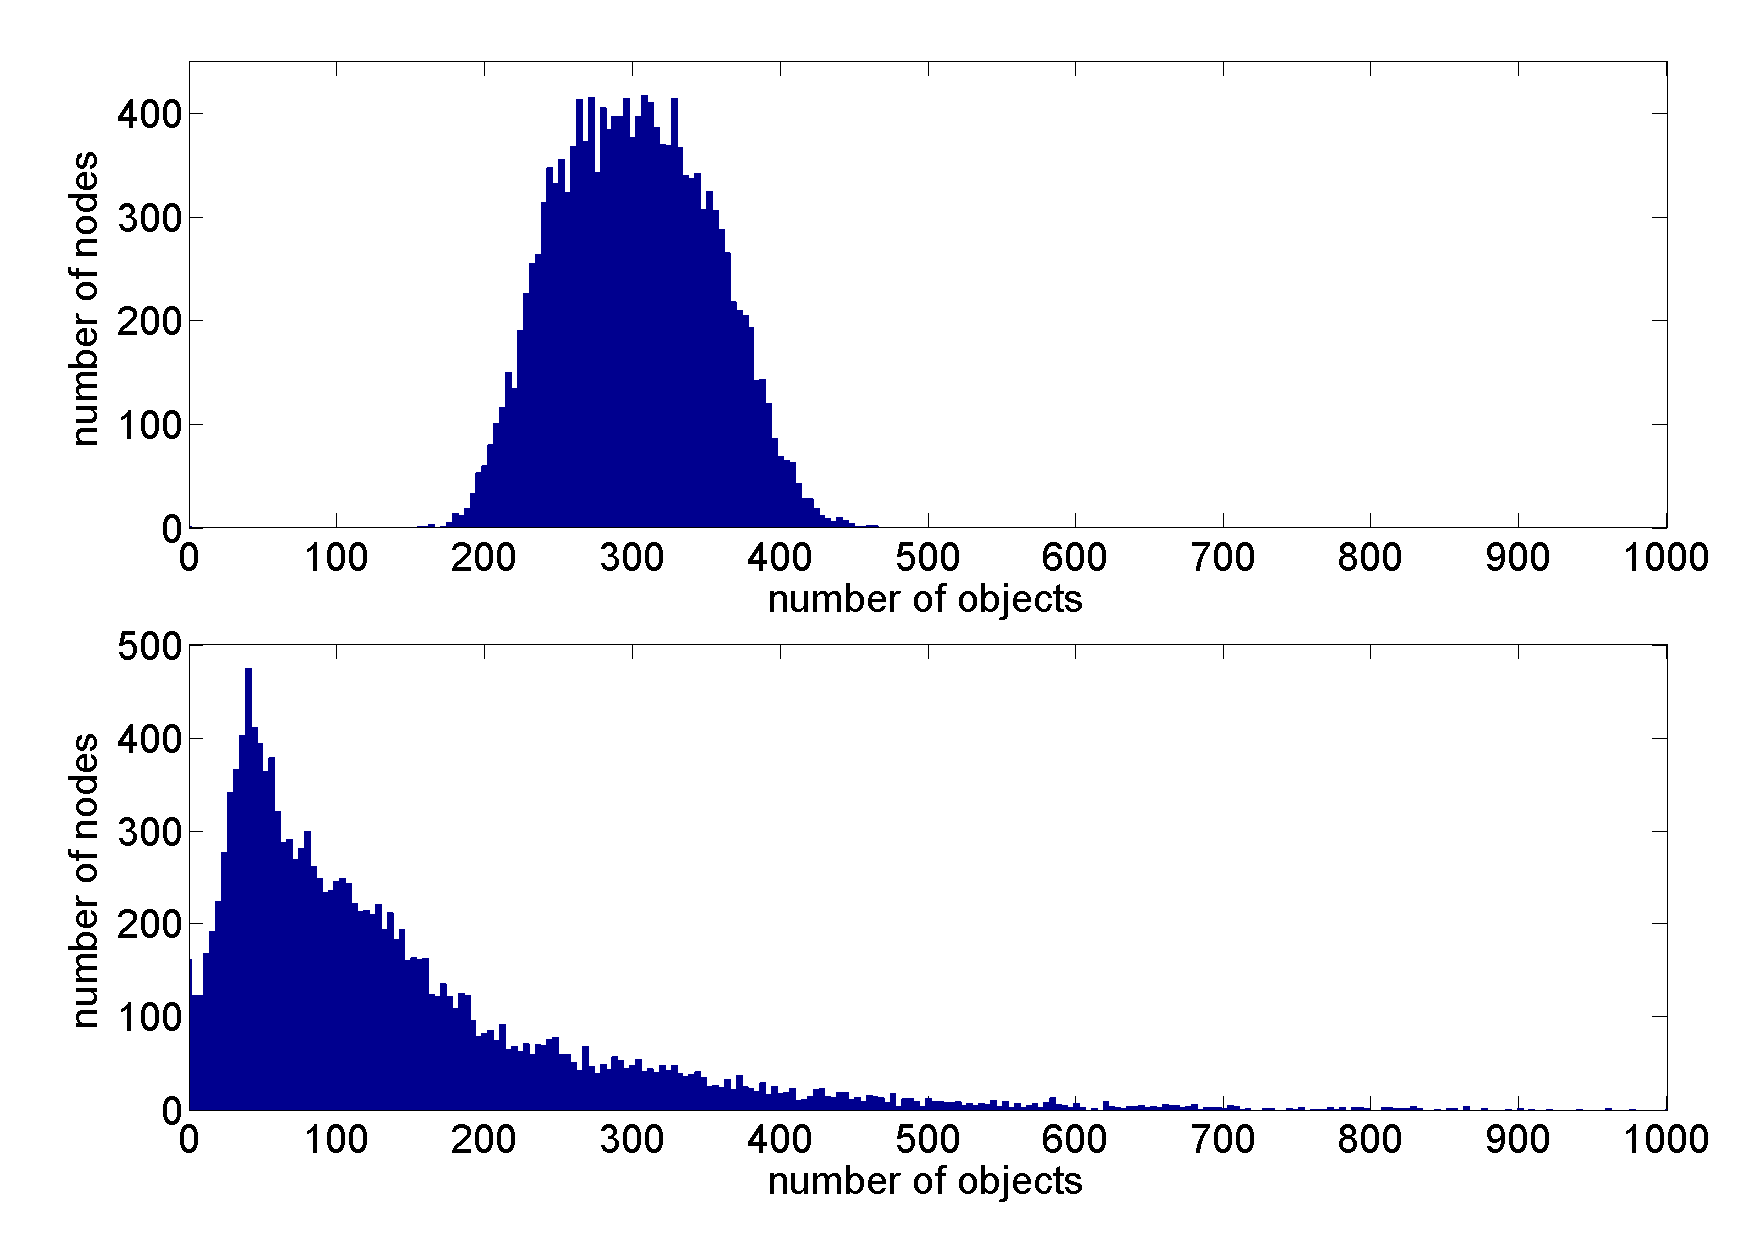
\includegraphics[clip=true, viewport=1cm 0.5cm 28.5cm 20cm, width=\columnwidth]{RootRepOverlayObjects}
 \caption{Root/Replica object number distribution}
 \label{fig_group_overlay_objects}
\end{figure}
%
To evaluate the fairness, we evaluate the standard deviation of the number of objects stored per peer. Figure \ref{fig_group_overlay_objects} (top)
shows the distribution of group objects over nodes in the network. The figure shows how many nodes store how many objects. From this figure it is
evident that the object distribution forms a Rayleigh distribution, with a mean and standard deviation of 302 and 51 objects per node respectively.

Figure \ref{fig_group_overlay_objects} (bottom) shows the distribution of overlay objects in Pithos with a mean and standard deviation of 153 and 189
objects per node respectively. Comparing the standard deviations of group storage to overlay storage, it is evident that group storage is much fairer
than overlay storage. This shows that by designing a hybrid system which prefers group storage to overlay storage, one is also designing a fairer
system than overlay storage.

At first glance, one might think that mapping one uniform distribution (the file ID hashes) to another uniform distribution (the node ID hashes) in a
distance-based manner of overlay storage would produce a system where the number of files per node is roughly balanced
\cite{storage_and_chaching_PAST}. This is not the case.

\begin{figure}[htbp]
 \centering
 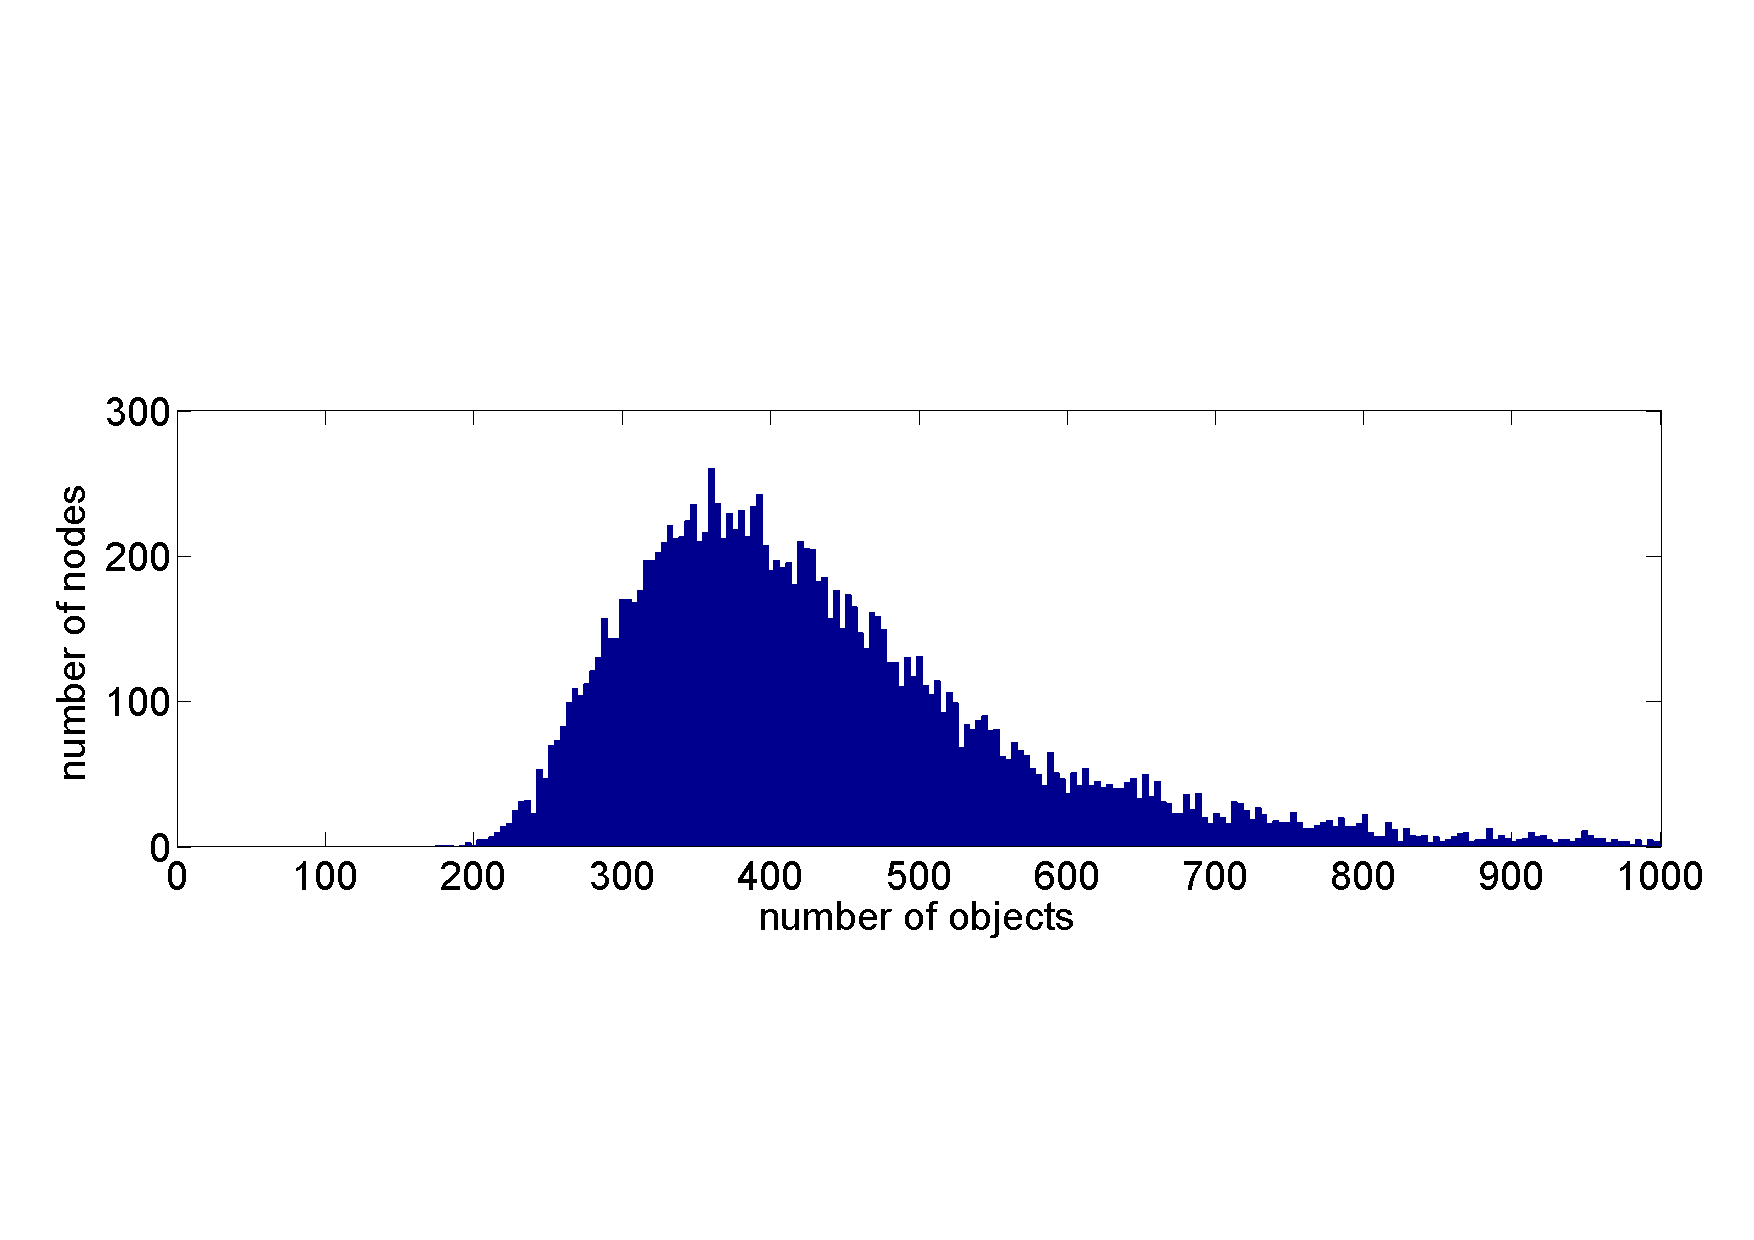
\includegraphics[clip=true, viewport=1cm 5cm 29cm 14.5cm, width=\columnwidth]{Objects}
 \caption{Combined object number distribution}
 \label{fig_objects}
\end{figure}
%
Figure \ref{fig_objects} shows the combined object distribution of Pithos, with a mean and standard deviation of 453 and 200 objects per node
respectively. This shows that the fairness of Pithos is currently dominated by the fairness of Pastry and that Pithos is as fair as overlay storage.

\section{Conclusion}
\label{conclusion}

\subsection{Summary}

In this paper, we presented a novel classification of storage types. None of the storage types satisfied all identified requirements of P2P MMVE
storage systems. A novel storage architecture called Pithos was presented to satisfy all the identified requirements, followed by a description of
all its key design aspects. For preliminary results, the requirements of responsiveness and reliability were compared to those of overlay storage and
Pithos was found to be more responsive than overlay storage and as fair.

\subsection{Future work}
\label{future_work}

%Complete implementation
For future work, we plan to complete the Pithos architecture and compare all requirements with all identified storage types. The simulation does not
yet support network churn. A migration mechanism should still be implemented before testing under churn can be done. Various improvements to the
current Pithos architecture can also be made. This includes using signalling to store files as described in Section \ref{store_retrieve} as well as
further improving fairness and responsiveness in Pithos.

A key aspect of completing Pithos will be how players are grouped. Future research will focus on player behaviour, clustering algorithms and dynamic
regioning approaches. The different clustering techniques should be compared and the most applicable one will be chosen to drive Pithos.


%Driver data
A model of data storage and retrieval requests are also required for a typical MMVE. This should include object sizes stored, how regularly these
objects are stored and what latency requirements exist for object retrieval. It is assumed that this will be very dependant on the specific MMVE and
therefore different storage parameters should also be identified. So although values used in this paper might be artificial, the comparisons of
responsiveness and fairness were still made between two systems with the same artificial values.


%\newpage
% use section* for acknowledgement
\ifCLASSOPTIONcompsoc
  % The Computer Society usually uses the plural form
  \section*{Acknowledgments}
\else
  % regular IEEE prefers the singular form
  \section*{Acknowledgment}
\fi

The financial assistance of MIH and the National Research Foundation (NRF) towards this research is hereby acknowledged. Opinions expressed and
conclusions arrived at, are those of the author and are not necessarily to be attributed to MIH or the NRF.

%\newpage
%\IEEEtriggeratref{43} %Balance the bibliography
\bibliographystyle{IEEEtran}
\bibliography{../BibTeX/P2P_MMOG}

% that's all folks
\end{document}
